\documentclass{article}
% Choose a conveniently small page size
% PACKAGES
\usepackage[margin = 1in]{geometry}
\usepackage{amsfonts}
\usepackage{amsmath}
\usepackage{amssymb}
\usepackage{multicol}
\usepackage{graphicx}
\usepackage{float}
\usepackage{xcolor}
\usepackage{amsthm}
\usepackage{dsfont}
\usepackage{hyperref}
\usepackage{listings}
\usepackage{subcaption}

\lstset{
  language=Python,
  basicstyle=\ttfamily\small,
  keywordstyle=\color{blue},
  stringstyle=\color{red},
  commentstyle=\color{olive},
  morecomment=[l][\color{magenta}]{\#},
  showstringspaces=false
}

% MACROS
% Set Theory
\def\N{\mathbb{N}}
\def\R{\mathbb{R}}
\def\C{\mathbb{C}}
\def\Z{\mathbb{Z}}
%\def\^{\hat}
\def\-{\vec}
\def\d{\partial}
\def\!{\boldsymbol}
\def\X{\times}
%\def\-{\bar}
\def\t{\text}
\def\b{\textbf}
\def\l{\left}
\def\r{\right}
\title{Weekly Report}
\author{Damien}
\begin{document}
\maketitle
% \newpage
\section{Summary}
I have a tentative implementation for the sweeping method on the Boltzmann equation. The code does not converge successfully yet and I am still in the process of debugging. However, I believe that I am close to having a working implementation. If you want to view the code it is available on my GitHub under the \verb|boltzmann_research/boltzmann| folder.
\section{Quick Review}
Here I add a quick review of the problem we are solving to have everything in one place. Most of this is copied from my update in \verb|1_12_24.pdf|. I also filled in some details that this report was missing.
\subsection{Simplification of Boltzmann Equation for 2D Maxwell Molecules}
Since the collision kernel is constant we can simplify the above integral. Note that both $f$ and $\rho$ (this will be defined later) are functions of $\b x$ but we drop this dependence for convenience of notation.
    
\begin{equation} \label{eq:derivation}
    \begin{aligned}
        \mathcal{Q}(f,f)(\b v) = \int_{\mathbb{R}^d} \int_{S^{d-1}} \frac{1}{2\pi}[f(\b v_*') f(\b v') - f(\b v_*) f(\b v)] \t d \sigma \t d \b v_* =\\
        \int_{\mathbb{R}^d} \int_{S^{d-1}} \frac{1}{2\pi}f(\b v_*') f(\b v') \t d \sigma \t d \b v_* - \int_{\mathbb{R}^d} \int_{S^{d-1}} \frac{1}{2\pi} f(\b v_*) f(\b v) \t d \sigma \t d \b v_* = \\
        \mathcal{Q}^+(f,f)(\b v) - \frac{1}{2\pi} f(\b v) \int_{\mathbb{R}^d} \int_{S^{d-1}}  f(\b v_*) \t d \sigma \t d \b v_* =\\ 
        \mathcal{Q}^+(f,f)(\b v) - \frac{1}{2\pi} f(\b v) \int_{\mathbb{R}^d} 2 \pi f(\b v_*) \t d \b v_* =\\
        \mathcal{Q}^+(f,f)(\b v) - C \rho f(\b v)
    \end{aligned}
\end{equation}


The constant $C$ comes from rescaling that is done in the derivation of the Boltzmann equation. This can be observed in \href{https://gyu-eun-lee.github.io/academic/gso_boltzmann.pdf}{this article}. The $\rho$ comes from the fact that we are integrating out velocity from the phase space probability function $f$ which leaves us with only the spatial density, $\rho$.
\subsection{Normal Shock Problem}
We will tackle the normal shock problem as stated in section 5.2 of Hu et al. \cite{hu2021adaptive}. We take $R=1$, $d=2$, hence $\gamma=2$, $M_L=u_L / \sqrt{2T_L}$. In the following, the spatial domain is chosen as $x_1 \in [-30,,30]$ with $N_{\b x} = 1000$; and the velocity domain is $(v_1,v_2) \in [-L_{\b v},L_{\b v}]^2$.

We choose the upstream and downstream conditions as
\[
    (\rho_L,\rho_R) = \left( 1, \frac{3M_L^2}{M_L^2 + 2}\right), \quad
    (u_L, u_R) = \left(\sqrt{2} M_L, \frac{\rho_L u_L}{\rho_R}\right), \quad
    (T_L, T_R) = \left(1, \frac{4M_L^2 - 1}{\rho_R} \right)
\]
and the downstream conditions as
\[
    \rho_0(x_1) = \frac{\tanh(\alpha x_1) + 1}{2(\rho_R - \rho_L)} + \rho_L, \quad
    T_0(x_1) = \frac{\tanh(\alpha x_1) + 1}{2(T_R - T_L)} + T_L, \quad
    \b u_0(x_1) = \left(\frac{\tanh(\alpha x_1) + 1}{2(u_R - u_L)}, 0 \right), \quad
\]
with $\alpha = 0.5$.

When showing the numerical results, we are mainly interested in the macroscopic quantities: density $\rho(x_1)$, bulk  velocity $u(x_1)$ ,and temperature $T(x_1)$. Their normalized calues will be plotted, which are defined by
\[
    \hat \rho(x_1) = \frac{\rho(x_1) - \rho_L}{\rho_R - \rho_L}, \quad
    \hat u(x_1) = \frac{u(x_1) - u_L}{u_R - u_L}, \quad
    \hat T(x_1) = \frac{T(x_1) - T_L}{T_R - T_L}.
\]

The initial condition for the phase space density function is

\[
    f_0(x_1, \b v, t) = \frac{\rho_0}{(2 \pi R T_0)^{d/2}} \exp \l(- \frac{(v_1 - u_0)^2 + v_2^2 + \hdots + v_d^2}{2 R T_0}\r)
\]

In Hu et al. \cite{hu2021adaptive} there is an example of a strong as well as a weak shock. We will model both of these.
\subsection{Numerical Scheme for the Normal Shock Problem}
For our numerical scheme we will be applying the methods developed in Chen et al. \cite{CHEN2013452} and applying them to the equation described above. For the left-to-right sweep the numerical discretization is 
\[
    \frac{v + |v|}{2} \frac{f_i^{(l+1)} - f_{i-1}^{(l+1)}}{\Delta x} + \frac{v - |v|}{2} \frac{f_{i+1}^{(l)} - f_i^{(l+1)}}{\Delta x} = Q^+(f^{(l)}, f^{(l)}) - C \rho_i^{(l)} f_i^{(l+1)}
\]
and for the right-to-left sweep the numerical discretization is
\[
    \frac{v + |v|}{2} \frac{f_i^{(l+1)} - f_{i-1}^{(l)}}{\Delta x} + \frac{v - |v|}{2} \frac{f_{i+1}^{(l+1)} - f_i^{(l+1)}}{\Delta x} = Q^+(f^{(l)}, f^{(l)}) - C \rho_i^{(l)} f_i^{(l+1)}.
\]
The update rule is acquired by isolating $f_i^{(l+1)}$ on one side.
\section{Progress}
I implemented the above method in Python. There is still a bug or two in the code and things are blowing up. I have parsed through my code carefully to check for any sort of typo. I could not find any. My issues are likely due to some misunderstanding that I have as opposed to a simple arithmetic error. Here I outline the details of my code to illustrate my understanding and how I chose to implement the method. All the code can be found under the \verb|boltzmann| folder on my GitHub repository. \textcolor{red}{Add GitHub link}
\subsection{Validation of Integration Scheme}
The first and easiest thing to validate were my integration schemes for recovering the density, bulk velocity, and temperature of the solution. Recall that 

\[
    \int_{\mathbb{R}^d} f(\b x, \b v, t)
    \begin{bmatrix}
        1 \\
        \b v \\
        \frac{1}{2} |\b v|^2
    \end{bmatrix}
    \t d \b v
    =
    \begin{bmatrix}
        \rho(\b x, t)\\
        \rho(\b x, t) \b u(\b x, t)\\
        \frac{1}{2} \rho(\b x, t) |\b u(\b x, t)|^2 + \frac{d}{2} \rho(\b x, t) R T(\b x, t)
    \end{bmatrix}.
\]

We use these formulas to recover the density, bulk velocity, and temperature of the solution. In the following plots we confirm that my methods for computing the integrals are accurate.

\begin{figure}[H]
    \centering
    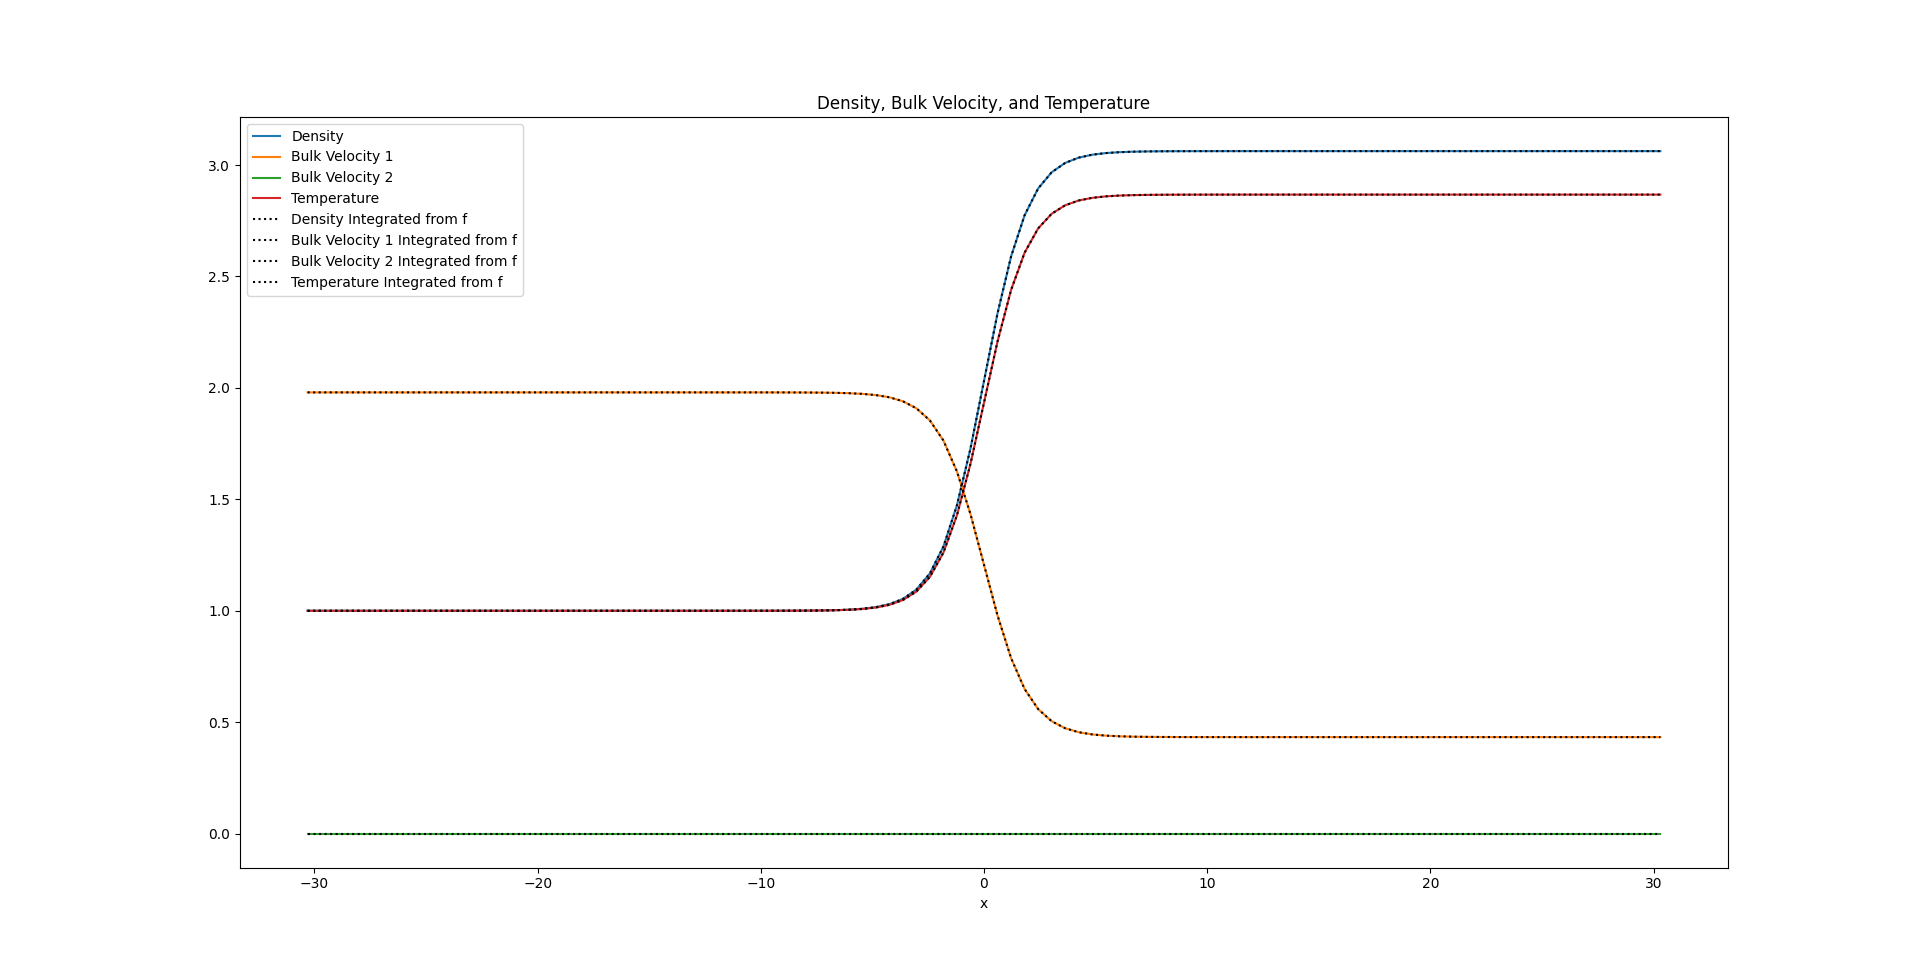
\includegraphics[width = \textwidth]{imgs/initial_distributions.png}
    \caption{The solid lines are the initial distributions for the the density, bulk velocity, and temperature. The dotted lines are the curves that we recover after integrating the phase space density function, $f$.}
\end{figure}

\subsection{Potential Problem Areas}
There are three places where I may have gone wrong with my code. In each of the following three sections I outline what I did in each of these sections to help expedite the identification of the issue.

\subsubsection{Scaling of Phase Distribution Function}
When the velocity is integrated out of $f_0$, we recover $\rho_0$. $\rho_0$ is the physical density of the system and not a probability density. This implies that $f_0$ is not a probability distribution in the phase space. This is contrary to what I had believed previously. Should $f$ be a physical density function or a probability density function? If $f$ is supposed to be a probability density then how do we determine the total mass of the system? Furthermore, since $\int f(\b x, \b v, t) \t d \b v$ integrates to $\rho(\b x, \b v, t)$ I set $C=1$ in Equation \ref{eq:derivation}.

\subsubsection{Collision Operator}

I changed the code in \verb|CBoltz2_Carl_Maxwell| slightly to return only the gain term of the collision operator as opposed to the entire collision operator. I call this adjusted function \verb|Q_plus|. \bigskip

\begin{lstlisting}
def Qplus(f, N, R, L, Ntheta):
    """
    Carleman spectral method for the classical Boltzmann collision operator
    2D Maxwell molecule
    N # of Fourier modes: f(N,N), Q(N,N)
    theta: mid-point rule
    """
    temp = np.concatenate((np.arange(0,N//2),np.arange(-N//2,0,1)))
    l1 = np.array([[row]*N for row in temp])
    l2 = l1.T
    
    FTf = fft2(f)

    QG = np.zeros((N, N), dtype=np.complex_)
    bb = np.zeros((N, N), dtype=np.complex_)

    wtheta = np.pi / Ntheta
    theta = np.arange(wtheta / 2, np.pi, wtheta)
    sig1 = np.cos(theta)
    sig2 = np.sin(theta)

    for q in range(Ntheta):
        aa1 = alpha2(l1 * sig1[q] + l2 * sig2[q], R, L)
        aa2 = alpha2(np.sqrt(l1**2 + l2**2 - (l1 * sig1[q] + l2 * sig2[q])**2), R, L)

        QG += 2 * wtheta * ifft2(aa1 * FTf) * ifft2(aa2 * FTf)
        bb += 2 * wtheta * aa1 * aa2

    # Original code #################
    # QL = f * ifft2(bb * FTf)
    # Q = np.real(QG - QL)
    #################################

    # Adjusted code #################
    Q = np.real(QG)
    #################################

    return Q
\end{lstlisting}
\bigskip
We do this so that we can make the stepping method implicit as we see in the next section.
\subsubsection{Sweeping Method}
The second source of error is in the sweeping method. I will describe this method for the case where $v>0$ to simplify notation. For the forward direction this gives

\[
    v \frac{f_i^{(l+1)} - f_{i-1}^{(l+1)}}{\Delta x} = Q^+(f^{(l)}, f^{(l)}) - C \rho_i^{(l)} f_i^{(l+1)}.
\]

Re-arranging terms we end up with

% \begin{equation}\label{eq:step}    
%     f_i^{(l+1)} = \l( \frac{\t d x}{v} + \frac{1}{C \rho^{(l)}_i}\r) Q^+ \l(f^{(l)}, f^{(l)}\r) + \l(1 + \frac{v}{C \rho_i^{(l)} d x} \r) f_{i-1}^{(l+1)}.
% \end{equation}
\begin{equation}\label{eq:step}    
    f_i^{(l+1)} = \l(1 + \frac{C \rho_i^{(l)} \Delta x}{v}\r)^{-1} \l( \frac{\Delta x}{v} Q^+ \l(f^{(l)}, f^{(l)}\r) + f_{i-1}^{(l+1)} \r).
\end{equation}

    All the tests I have run have been with $C=1$ and $v=1$. Let's put this in Python notation to be as clear as possible about how the computation works. In the algorithm, \verb|f| is a $1001 \times 32 \times 32$ array. The first dimension is the spatial dimension and the other dimensions are velocity dimensions. We use the line \verb |Qplus_grid = get_Qplus_grid(f,Nv,R,Lv,Ntheta)| to get the gain term in the collision operator at every point in phase space. The \verb|get_Qplus_grid| function applies the \verb|Qplus| function to $f$ for each x-value on the grid. The code is the following.

\bigskip
\begin{lstlisting}
def get_Qplus_grid(f,Nv,R,Lv,Ntheta): # get the gain term of the collision operator on the grid
    Q_plus_grid = np.empty(f.shape)
    for i in range(f.shape[0]):  # Iterate over the second dimension.
        Q_plus_grid[i,:,:] = Qplus(f[i,:,:],Nv,R,Lv,Ntheta)
    return Q_plus_grid
\end{lstlisting}
\bigskip
\verb|Qplus| is a $1001 \times 32 \times 32$ array, same as \verb|f|. Translating Equation \ref{eq:step} into code we get
\bigskip
\begin{lstlisting}
def sweep(f,p,Qplus_grid,v,C,dx,n): # sweeping method for the Boltzmann equation
    # Forward Sweep
    for i in range(1,n):
        f[i,:,:] = ((dx/v) * Qplus_grid[i,:,:] + f[i-1,:,:])/(1 + (C * p[i] * dx)/v)
    # Backward Sweep
    for i in range(n-1,0,-1):
        f[i,:,:] = ((dx/v) * Qplus_grid[i,:,:] + f[i-1,:,:])/(1 + (C * p[i] * dx)/v)
    return f
\end{lstlisting}

\subsection{Results}

The code runs and does not immediately break. However, the density function quickly starts to diverge as one can observe in the following images.
\bigskip

\begin{figure}[h]
    \centering
    \begin{subfigure}[b]{0.45\textwidth}
    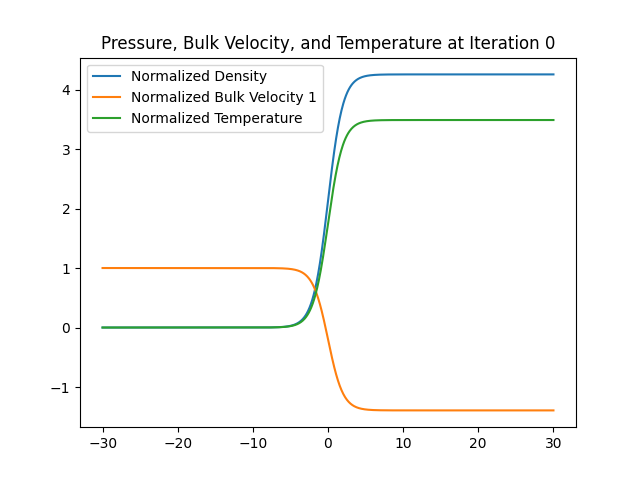
\includegraphics[width=\textwidth]{imgs/iter0.png}
        % \caption{Image 1}
        \label{fig:image1}
    \end{subfigure}
    \hfill
    \begin{subfigure}[b]{0.45\textwidth}
    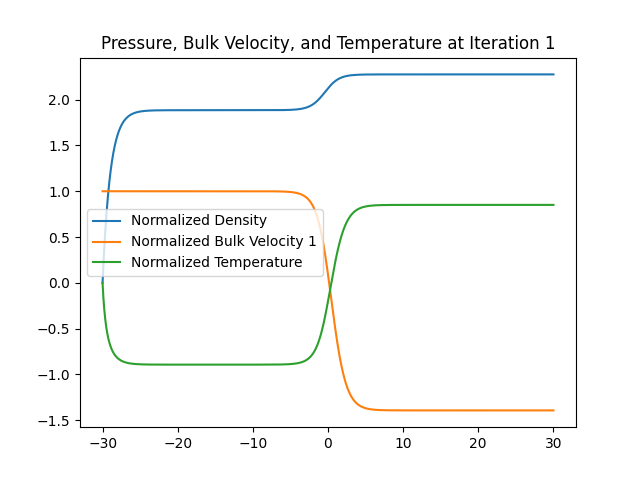
\includegraphics[width=\textwidth]{imgs/iter1.png}
        % \caption{Image 2}
        \label{fig:image2}
    \end{subfigure}
    
    \vspace{1em} % Add some vertical space between the rows
    
    \begin{subfigure}[b]{0.45\textwidth}
    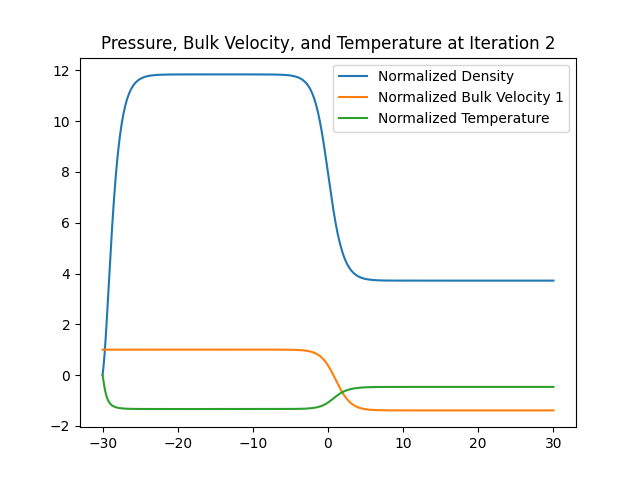
\includegraphics[width=\textwidth]{imgs/iter2.png}
        % \caption{Image 3}
        \label{fig:image3}
    \end{subfigure}
    \hfill
    \begin{subfigure}[b]{0.45\textwidth}
    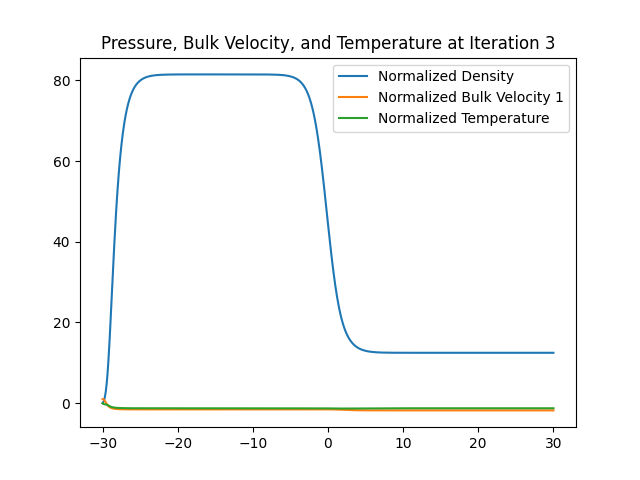
\includegraphics[width=\textwidth]{imgs/iter3.png}
        % \caption{Image 4}
        \label{fig:image4}
    \end{subfigure}
    
    \caption{The above plots show the normalized density, bulk velocity, and temperature from the normal shock problem. These plots should ideally converge to look like the right plot in Figure 2 for \cite{hu2021adaptive}. However, the density function continually grows without bound. All experiments were done with $v=1$}
    \label{fig:four_images}
\end{figure}

\section{To Do}
The main priority is to debug the code. I have some ideas for how to diagnose what is going wrong with the code.
\begin{enumerate}
    \item I could forget the sweeping method and solve the time-dependent equation to ensure that it works correctly
    \item I can explore the value of the Knudsen number. There is perhaprs some scaling that I am not accounting for
    \item I can make test cases for the collision operator function in python to ensure that my adjusted function is correct
    \item I can take out the collision operator to see whether the method converges to a constant steady state as it should 
\end{enumerate}
Once this is done I plan to implement the shock problem given to me by Jingwei two meetings ago.
\bibliographystyle{plain}
\bibliography{refs}
\end{document}